\section{Motivation} \label{sec:motivation}
% Programming a legacy network control plane to satisfy a variety of
% connectivity, security, and performance policies is a complex and error-prone
% task. We have shown that program synthesis is a promising approach to automate
% this process and produce a control plane that is ``correct-by-construction.''
% In particular, we presented an architecture where a network operator provides
% a policy-compliant data plane and a set of hard and soft policies as input,
% and the system automatically provides a set of device configurations that
% leverage the control plane features available on each device to compute
% policy-compliant paths, even in the presence of failures.  Formulating a
% tractable synthesis problem and maximizing the number of satisfied soft
% policies are the key challenges in realizing this vision. We show these
% challenges can be overcome by modeling the control plane using a graph-based 
% abstract representation tied to a traditional shortest path algorithm and
% iteratively transforming the abstract representation based on feedback from
% the satisfiability (SAT) solver and characteristics of the graph. However, we
% have only explored how to address a subset of important policies and leverage a
% few available control plane features on traditional networking hardware. Our
% future work will focus on satisfying a wider range of policies using more
% features, and we will study how to best translate our abstract representation
% into actual device configurations to make our system practical for use with
% real networks.

One of the foremost tasks in network management is programming the network to
forward traffic in a manner consistent with user- and application-induced
policies. Common types of policies include: reachability (i.e., which
end-hosts can communicate), isolation (i.e., which flows cannot share links),
service chaining (i.e., which middleboxes must be traversed), resilience
(e.g., how many backup paths are available), and traffic engineering 
objectives like minimizing the average link utilization. Every
set of forwarding paths (i.e., data plane) installed in the network
%---either manually or by a control plane---
should conform to these 
policies, otherwise performance, security, or availability problems may arise.

% A variety of techniques can be used to determine the appropriate forwarding
% paths. One option is to compute a data plane offline, and install the data
% plane using an API that allows direct control of switches' forwarding tables
% (e.g., OpenFlow). Several recent works~\cite{merlin} have adopted this
% approach, using solvers to automatically compute a data
% plane that conforms to a set of policies. 
% A second option is to dynamically compute forwarding
% paths at a logically centralized controller---i.e., use a software-defined
% networking (SDN) control plane. However, this requires developing algorithms
% that take the set of policies and the current state of the network (e.g.,
% which links have failed) as input and output paths that conform to a
% multiplicity of policies.  Most existing SDN control applications only compute
% paths based on one or a few types of policies: e.g., service
% chaining~\cite{simple, flowtags}, traffic engineering~\cite{swan, b4}, or
% resilience~\cite{plinko}. Furthermore, in both approaches, the centralized policy
% component may become bottlenecked
% or fail (even if it is distributed), leading to (a partial) network failure.

A common theme among these policies is that 
they specify \emph{network-wide intent}~\cite{intent},
operators can specify what they \emph{want} from the network as a 
whole, instead of \emph{how} individual components of the network
must be configured. 
Software-defined networking (SDN) has led to the development 
of various frameworks for network-wide policy enforcement
~\cite{netkat, simple, merlin, fattire, genesis}. In SDN,
a centralized controller machine (control plane) controls
the end-to-end paths by managing forwarding rules on programmable
network switches (data plane). The controller can program
forwarding rules using the global view of the network
topology to meet application requirements. While SDN 
significantly enhances programmability of the network to 
satisfy the diverse policy requirements in multi-tenant
clouds and enterprise networks, it suffers from two 
major challenges: 
\emph{scalability} and \emph{fault tolerance}. 

The centralized controller is responsible for installing 
forwarding rules to all switches, and thus, as network sizes
increase, the overhead of rule installation could increase
significantly. When a network failure (link/switch) occurs,
the controller has to detect and respond to the failure, and
even establishing connectivity between endpoints could be delayed.
Also, the controller is a central point of failure and controller
failure can lead to network disruptions. 
The principles of scalability and fault tolerance 
were instrumental to the design
of 'traditional' networks (e.g., the Internet) using distributed
routing protocols like OSPF and BGP to manage forwarding in the 
network without a central control entity. Another reason for the 
slow adoption of SDN has been the cost involved in overhaul 
of the network with programmable switches.  

Unlike SDN which provide a clean abstraction
to program the network to satisfy policies 
on end-to-end paths,
programming (i.e., configuring) 
routers such that the paths computed by
the distributed routing protocols enforce the 
policies is challenging for several reasons: 
\setlist[itemize]{
    topsep=.5ex,
    itemsep=0ex,
    leftmargin=1em,
}
\begin{itemize}
%\setlength{\topsep}{0ex}
%\setlength{\itemsep}{0ex}
%\setlength{\parskip}{0pt}
%\setlength{\parsep}{0pt}
\item The available path-computation algorithms
available are predefined---e.g., OSPF uses
Dijkstra's shortest path---and their behavior can only be influenced
through a limited set of parameters---e.g.,
link weights. Similarly, BGP uses shortest
path routing at a domain-granularity, and have different
provisions to control routing (like local preferences).  
\item Operators can have 
heteregeneous protocol requirements based on operational
factors like scalability and cost, thus requiring to model
protocol interactions. 
\item Most policies are
global---i.e., they concern end-to-end paths, not individual devices and
links---making it difficult to map policies to
individual router configurations. 
\item Since fault tolerance is handled in a distributed 
fashion with no involvement of a central control entity,  
fault tolerance properties like resilience under bounded
number of network failures must be taken into account in
the generation of router configurations. 

%A single set of parameters must result in
%policy-compliant paths under all reasonable network states---e.g., a bounded
%number of link failures.
\end{itemize}

\begin{figure*}
\centering
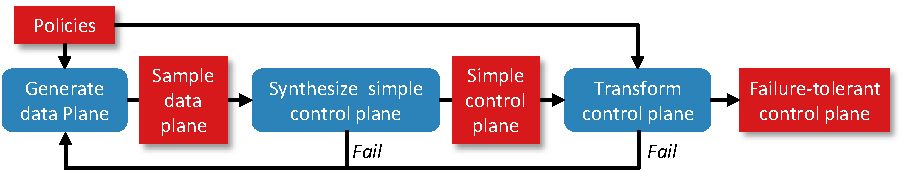
\includegraphics[width=0.7\textwidth]{figures/process.pdf}
\caption{Three-phase process for generating a control plane that generates
    policy-compliant paths under bounded failures}
\label{fig:process}
\end{figure*}

\subsection{Architecture}

These issues motivate us to design a 
system that automatically synthesizes
(configurations for) a control plane that computes policy-compliant paths
under a bounded number of failures.
Unfortunately, this task is inherently challenging as it requires solving in one shot multiple
computationally hard problems.
For example, even when considering static routing and no failures, synthesizing a control plane that satisfies  policies such as isolation and waypoints
is an NP-hard problem.
Although the progress in SMT solving has made many NP-hard problems more practical, 
attempts of incorporating concepts such as shortest path algorithms 
into these solvers have resulted into huge performance losses~\cite{monosat}. 
Finally, adding failure handling to the problem results in yet another layer of combinatorial explosion.
Our proposed approach is to tackle these three problems in separate phases
(\figref{fig:process}).
First we synthesize a data plane that meets the input policies and then,
by using the data plane as input to the second phase, we 
express the problem of finding a policy-compliant control plane using only the 
theory of linear rational arithmetic (LRA), for which we can use
efficient off-the-shelf LP-solvers. 
Finally, we modify the obtained control plane to obtain failure tolerance.
The drawback of this approach is that one might need to consider multiple possible
data planes before finding one that can successfully complete all the phases of the
synthesis algorithm
%ailures that happen in the later phases may require to restart the synthesis procedure 
%multiple times.
%but preliminary results of our approach are promising.

The solution space of output network configurations to 
enforce a set of policies
is large; configurations can use different 
network protocols (e.g., only BGP, only OSPF or a hybrid) and
mechanisms (e.g., route filters, access control lists
or protocol-specific variables). The large solution space
of configurations complicates the synthesis of
network configurations from
input policies, 
or ties the synthesis to a particular type of configuration. 
Instead, we borrow a page from programming languages
research and
synthesize an Abstract Representation for Control planes (ARC)~\cite{arc} 
from the data plane; the ARC can then be translated to actual device configurations.
The ARC uses the notion that most routing protocols in use 
today employ a cost-based path selection algorithm; thus a weighted
graph can be used to abstractly represent the control plane such that 
the path between two points taken in the network would be 
the lowest weight path in the graph. 
The ARC effectively decouples the policy component with the 
actual network infrastructure. 

% While we use an abstract representation of the control
% plane (ARC) to simplify the synthesis, operators need control 
% planes conforming to certain requirements of the 
% underlying network infrastructure. For example, a 
% network may comprise of switches which do not have custom
% features like ACLs or route-filters, thus the ARC must take 
% into consideration these requirements. Without losing 
% generality, we translate these 
% requirements as types of ARCs with different properties,
% and still use a protocol-independent representation
% to represent the control plane. 

% In this paper, we primarily focus on 
% the second and third phase of our architecture, 
% i.e synthesizing a control plane from a set 
% of input paths and transforming the control plane to 
% satisfy policies under failure scenarios. The first 
% phase has seen promising work in recent times~\cite{merlin,
% simple}, these systems generate data planes to enforce 
% different kinds of policies, and 
% we can be retrofit these systems to generate different 
% data planes to integrate in our three-phase approach.

% thus, the networking infrastructure could be
% transitioned to different protocols without affecting the policy 
% control of the architecture. From the ARC, we can construct different
% drivers for translation to actual device configurations; these drivers
% can leverage inferences from healthy network practices in 
% real-life networks~\cite{mpa-imc15} to produce ideal network configurations.


%\aaron{Old text below}
%
%To tackle synthesis 
%of distributed control planes, 
%we use as input the network data plane 
%(set of forwarding paths) \aaron{Where does this data plane come from and
%    why is it reasonable to assume an operator can provide one?} which 
%enforces the operator-specified policies to
%synthesize an abstract representation of the control plane
%called ARC. \aaron{Our approach (ARC) should not come up until later in the
%    motivation, if at all.}
%The advantage of using network data planes as 
%input is the ease of developing
%different network management applications 
%enforcing proactive policies\footnote{
%Traditional control planes cannot support reactive policies, however
%middleboxes can overcome this limitation.} 
%as if operating over a software-defined
%network, agnostic of the actual network protocols used in the network.
%\aaron{I don't understand the preceding sentence. I'm still not clear why you
%take a single data plane as input and not multiple data planes or just the
%policies. I realize it is hard to synthesize from the latter, but can you be
%more precise why it is hard?}
%Many existing network management systems like Merlin~\cite{merlin} 
%and SIMPLE~\cite{simple}\footnote{
%Traditional control planes cannot support 
%paths with loops for service chaining.} developed for SDNs 
%could be seamlessly integrated to the architecture with minimal changes.
%\aaron{Do we need the preceding sentence?}
%Thus, using the data plane as input, we synthesize a control plane
%such that the paths decided by the control plane are the same 
%as the data plane input, and these paths satisfy the operator 
%policies.
%
%However, the control plane does not guarantee policy compliance 
%when failures occur. For
%example, if a link along the shortest path 
%%(\aaron{refer to some example figure}) 
%fails, \aaron{Need to mention earlier that we assume shortest-path-based route
%computations, ala OSPF} the next shortest path will become the new path to reach the
%destination. The control plane automatically computes the new shortest path
%(assuming one exists), thus preserving connectivity. 
%However, the new path may
%not conform to the same policies as the path in the 
%original failure-free data
%plane from which the control plane was synthesized: 
%e.g., the new path may no longer
%traverse a waypoint or have the same bandwidth capacity. Thus,
%synthesis must take into account policy-compliance under failures.
%
%Policy-compliance under failures is difficult to achieve due 
%to the large number of failure scenarios to consider and can 
%be impossible to synthesize a control plane which is 
%policy-compliant under all failures. Operators require 
%varying degrees of policy-compliance under failures for 
%which we propose two classes of policies: {\em hard} and
%{\em soft} policies. Operators can specify 
%hard policies pertaining
%to security are of the utmost importance, 
%because they protect the network and
%its services from attacks and unauthorized accesses. Some 
%examples of hard policies are as follows: 
%a particular flow must always traverse through a waypoint 
%under any failure scenario, or a certain pair of hosts must 
%never be able to communicate (always blocked). 
%Soft policies can be considered as objectives which improve 
%the control plane, but are not strict requirements, typically
%pertaining to performance. The consequences of violating
%soft policies are less severe. Operators can provide 
%backup paths for flows (generated such that they 
%satisfy the data plane policies) as soft policies, 
%and the synthesis of the control plane 
%tries to satisfy as many soft policies as 
%possible. 
%
%\aaron{Discussion of the available control plane constructs should come up
%    earlier.}
%While we use an abstract representation of the control
%plane (ARC) to simplify the synthesis, operators need control 
%planes conforming to certain requirements of the 
%underlying network infrastructure. For example, a 
%network may comprise of switches which do not have custom
%features like ACLs or route-filters, thus the ARC must take 
%into consideration these requirements. Without losing 
%generality, we translate these 
%requirements as policies determining the properties of the
%ARC, and thus, still use a protocol-independent representation
%to represent the control plane. 
%
%Our architecture envisions network operator providing
%a policy-compliant data plane and a set of hard and soft policies
%pertaining to policy-compliance under failure and network 
%infrastructure requirements as input to synthesize resilient 
%control planes. Towards this vision, we present  
%approaches to synthesize different types of the ARC and the 
%challenges involved in making synthesis efficient and
%extending these approaches to support a wider range of 
%policies and functionalities. 
